%===================================================================================
% JORNADA CIENTÍFICA ESTUDIANTIL - MATCOM, UH
%===================================================================================
% Esta plantilla ha sido diseñada para ser usada en los artículos de la
% Jornada Científica Estudiantil, MatCom.
%
% Por favor, siga las instrucciones de esta plantilla y rellene en las secciones
% correspondientes.
%
% NOTA: Necesitará el archivo 'jcematcom.sty' en la misma carpeta donde esté este
%       archivo para poder utilizar esta plantila.
%===================================================================================



%===================================================================================
% PREÁMBULO
%-----------------------------------------------------------------------------------
\documentclass[a4paper,10pt,twocolumn]{article}

%===================================================================================
% Paquetes
%-----------------------------------------------------------------------------------
\usepackage{amsmath}
\usepackage{amsfonts}
\usepackage{amssymb}
\usepackage{jcematcom}
\usepackage[utf8]{inputenc}
\usepackage{listings}
\usepackage[pdftex]{hyperref}
%-----------------------------------------------------------------------------------
% Configuración
%-----------------------------------------------------------------------------------
\hypersetup{colorlinks,%
	    citecolor=black,%
	    filecolor=black,%
	    linkcolor=black,%
	    urlcolor=blue}

%===================================================================================



%===================================================================================
% Presentacion
%-----------------------------------------------------------------------------------
% Título
%-----------------------------------------------------------------------------------
\title{Proyecto de Lógica Difusa. Simulación.}

%-----------------------------------------------------------------------------------
% Autores
%-----------------------------------------------------------------------------------
\author{\\
\name Antonio Jesús Otaño Barrera \email \href{mailto:a.otano@estudiantes.matcom.uh.cu}{a.otano@estudiantes.matcom.uh.cu}
	\\ \addr Grupo C411}

%-----------------------------------------------------------------------------------
% Headings
%-----------------------------------------------------------------------------------
%\jcematcomheading{\the\year}{1-\pageref{end}}{A. Uno, A. Dos}

%-----------------------------------------------------------------------------------
%\ShortHeadings{Ejemplo JCE}{Autores}
%===================================================================================



%===================================================================================
% DOCUMENTO
%-----------------------------------------------------------------------------------
\begin{document}

%-----------------------------------------------------------------------------------
% NO BORRAR ESTA LINEA!
%-----------------------------------------------------------------------------------
\twocolumn[
%-----------------------------------------------------------------------------------

\maketitle

%===================================================================================
% Resumen y Abstract
%-----------------------------------------------------------------------------------
\selectlanguage{spanish} % Para producir el documento en Español


%-----------------------------------------------------------------------------------
% NO BORRAR ESTAS LINEAS!
%-----------------------------------------------------------------------------------
\vspace{0.8cm}
]
%-----------------------------------------------------------------------------------


%===================================================================================


\section{Características del sistema de inferencia propuesto}\label{sec:1}
%---------------------------------------------------------------------------------------------------------------------------------------------------------------------

  \paragraph{} El sistema de inferencia propuesto acepta reglas con  múltiples variables de entrada y múltiples variables de salida. Las variables
  en la entrada pueden ser tanto valores (singleton) como conjuntos difusos. El sistema permite trabajar con funciones de membresía
  de cualquier tipo definidas por el usuario, y además brinda herramientas para facilitar el uso de funciones membresía de tipo singleton, triangular
  y trapezoidal. Los métodos de inferencia que tiene implementados son los de Mamdani y Larsen, y los métodos de desdifusificación que
  brinda son los de Centroide (Center of Area), Bisección (Bisector of Area), y Media de los Máximos (Mean of Maximum).

%===================================================================================

\section{Principales ideas seguidas para la implementación del sistema}\label{sec:2}
%---------------------------------------------------------------------------------------------------------------------------------------------------------------------

  \paragraph{} El sistema fue implementado en Python y consiste en una librería que permite a cualquier otro programador usarla para
  resolver (siempre y cuando esté bien modelado) cualquier problema cuya solución se obtenga mediante inferencia difusa. El programador
  puede escoger el método de inferencia y el método de desdifusificación que más se ajuste al problema con que está tratando. Además, dado que
  el universo de discusión del problema puede ser continuo es necesario discretizar las funciones de membresía provistas por el usuario
  para poder efectuar tanto los métodos de inferencia como los de desdifusificación. La discretización que se realiza es uniforme y es tarea del
  programador definir el número de segmentos o niveles en que se divide el universo del problema original. También se puede proveer al sistema de
  una función para normalizar la entrada en un determinado rango. El sistema trabaja con cuatro entidades fundamentales: conjuntos difusos, variables
  linguísticas, reglas difusas y bases de reglas difusas. Estas entidades a su vez deben ser usadas por el programador para modelar su problema. Internamente solo
  se trabaja con reglas de tipo MISO (multiple input single output), pero como toda regla MIMO (multiple input multiple output) puede ser transformada en una conju
  nto de reglas de tipo MISO, se brinda una interfaz para modelar el problema con reglas MIMO, las cuales se descomponen internamente en varias reglas de tipo MISO.   

%===================================================================================

\section{Propuesta de problema a solucionar mediante inferencia difusa}\label{sec:3}
%---------------------------------------------------------------------------------------------------------------------------------------------------------------------

  \paragraph{}   El problema propuesto consiste en simular el movimiento de un robot sobre un espacio en el que existen obstaculos.
  El robot tiene sensores que le permiten detectar la distancia a la que se encuentra del objeto más cercano así como el ángulo que forma
  con el mismo. Conocidos estos parámetros el robot debe determinar que dirección tomar para evitar chocar con el obstáculo (Figura \ref{ex})
  
	\begin{figure}[htb]%
		\begin{center}
			\setlength\fboxsep{0pt}
			\setlength\fboxrule{1.5pt}
			\fbox{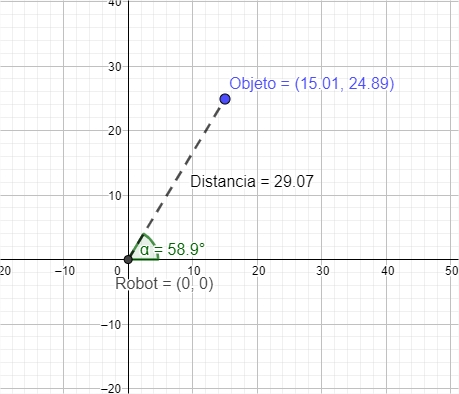
\includegraphics[width=200px, height=200px]{images/problem_description.jpg}}
		\end{center}
		\caption{Descripción del problema \label{ex}}%
	\end{figure}

\subsection{Variables linguísticas definidas}\label{sub:variables}
\paragraph{}A partir del enunciado anterior podemos definir tres variables lingüisticas que nos permitirán modelar el problema, como se muestra en la Tabla \ref{tab:lv}.

\begin{table}[htb]%
	\begin{center}
		 \begin{tabular}{| l | l | p{5.3cm} |}
			  \hline
			    Variable & Tipo & Términos \\ \hline
			    Distancia & Estado & muy cerca, cerca, un poco lejos, lejos, muy lejos \\ \hline
			    Ángulo & Estado & der-grande, der-mediano, \newline der-pequeño, nulo, izq-pequeño, izq-mediano, izq-grande \\ \hline
			    Dirección & Control & izq-cerrado, izq-moderado, \newline izq-leve, recto, der-leve, \newline der-moderado, der-cerrado \\ \hline
		  \end{tabular}
		  
		  \caption{Variables lingüisticas del problema  \label{tab:lv}}%
		 
	\end{center}
\end{table}

%\subsection{Variables linguísticas definidas}\label{sub:variables}

%===================================================================================



%===================================================================================
% Desarrollo
%-----------------------------------------------------------------------------------
\section{Desarrollo}\label{sec:dev}
%-----------------------------------------------------------------------------------
  En esta sección (o secciones) incluya el contenido fundamental del artículo.
  No es necesario tener una sección nombrada \emph{Desarrollo}, por el contrario,
  nombre las secciones según el contenido que tratan.

%-----------------------------------------------------------------------------------
	\subsection{Organización del Documento}\label{sub:results}
%-----------------------------------------------------------------------------------
		Puede agregar secciones y subsecciones según sea necesario para organizar
		de manera más coherente su artículo. Tenga en cuenta que un documento más
		plano es más fácil de navegar y entender, pero las subsecciones relacionadas
		deberían estar agrupadas en una sección común.

		Los nombres de las secciones deben ir en mayúsculas, excepto para las
		preposiciones, conjunciones, y otros vocablos auxiliares.

		Empiece un nuevo párrafo cada vez que vaya a comenzar una idea nueva.

%-----------------------------------------------------------------------------------
	\subsection{Listas y Descripciones}\label{sub:lists}
%-----------------------------------------------------------------------------------
		Para producir listas enumeradas, use el siguiente estilo:

%-----------------------------------------------------------------------------------
		\begin{enumerate}
			\item Primer Elemento
			\item Segundo Elemento
			%
			\begin {enumerate}
				\item {Segundo Elemento - Subitem Uno}
				\item {Segundo Elemento - Subitem Dos}
			\end {enumerate}
			%
		\end{enumerate}

%-----------------------------------------------------------------------------------
		Para producir descripciones, use el siguiente estilo:

%-----------------------------------------------------------------------------------
		\begin{description}
			\item [Primer Elemento] con su respectiva descripción.
			\item [Segundo Elemento] también con su respectiva descripción.
		\end{description}

%-----------------------------------------------------------------------------------
	\subsection{Figuras}\label{sub:figures}
	

%-----------------------------------------------------------------------------------
		Para producir cuerpos flotantes (figuras ó tablas), asegúrese de numerar
		y etiquetar correctamente cada figura. Las referencias a las figuras deben
		estar también correctamente etiquetadas. Por ejemplo, en la Fig. \ref{fig:arr}
		se muestra\ldots.

		\begin{figure}[htb]%
		\begin{center}
		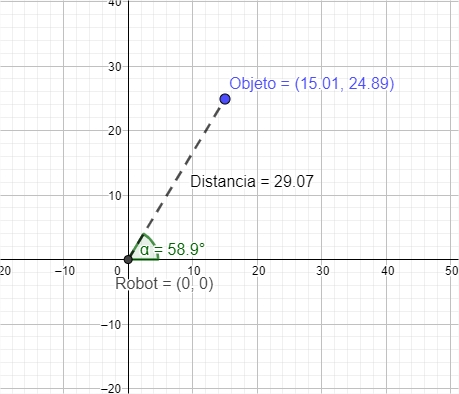
\includegraphics[width=200px, height=200px]{images/problem_description.jpg}
		\end{center}
		\caption{Descripción del problema \label{fig:arr}}%
		\end{figure}

%-----------------------------------------------------------------------------------
	\subsection{Código Fuente}\label{sub:listings}
%-----------------------------------------------------------------------------------
		Para producir código fuente, envuélvalo en una figura flotante y
		etiquételo correctamente. Por ejemplo, en la Fig. \ref{fig:code}
		se muestra un código bastante conocido\ldots.

		% Configuración de Listings
		\lstset{keywordstyle=\color{blue}, basicstyle=\small}

		\begin{figure}[htb]%
			\begin{lstlisting}[language=c]%

    int main(int argc, char** argv)
    {
        // Imprimiendo "Hola Mundo".
        printf("Hello, World");
    }

			\end{lstlisting}
		\caption{Código fuente de ejemplo.\label{fig:code}}
		\end{figure}

%-----------------------------------------------------------------------------------
	\subsection{Referencias}
%-----------------------------------------------------------------------------------
  	Las referencias deben estar agrupadas en una sección al final del artículo,
  	y las citas numeradas correctamente, por ejemplo \cite{knuth} ó \cite{goedel}.
  	Incluya toda la información importante de cada referencia, incluídos autor,
  	título, y notas de la edición. En caso de citar sitios web, además
  	de la URL, incluya la fecha en que fue consultado, como en \cite{wiki}.

%===================================================================================



%===================================================================================
% Conclusiones
%-----------------------------------------------------------------------------------
\section{Conclusiones}\label{sec:conc}

  En esta sección puede incluir las conclusiones de su investigación y las ideas
  sobre la continuidad del trabajo, en el caso que aplique.

%===================================================================================



%===================================================================================
% Recomendaciones
%-----------------------------------------------------------------------------------
\section{Recomendaciones}\label{sec:rec}

  En esta sección puede incluir recomendaciones sobre posibles formas de continuar
  la investigación u otros temas relacionados.

%===================================================================================



%===================================================================================
% Bibliografía
%-----------------------------------------------------------------------------------
\begin{thebibliography}{99}
%-----------------------------------------------------------------------------------
	\bibitem{knuth} Donald E. Knuth. \emph{The Art of Computer Programming}.
		Volume 1: Fundamental Algorithms (3rd~edition), 1997.
		Addison-Wesley Professional.

	\bibitem{goedel} Kurt Göedel. \emph{Über formal unentscheidbare Sätze der
		Principia Mathematica und verwandter Systeme, I}.
		Monatshefte für Mathematik und Physik 38.

	\bibitem{wiki} Wikipedia. URL: \href{http://en.wikipedia.org}
	  {http://en.wikipedia.org}.
		Consultado en \today.

%-----------------------------------------------------------------------------------
\end{thebibliography}

%-----------------------------------------------------------------------------------

\label{end}


\end{document}

%===================================================================================
